% ---------------------------------------------------
%
% Trabajo de Fin de Grado. 
% Author: Alejandro Hernández Padrón. 
% Capítulo: Tecnologías utilizadas en el Trabajo de Fin de Grado. 
% Fichero: Cap2_Technology.tex
%
% ----------------------------------------------------
%

\cleardoublepage
\chapter{Herramientas y Tecnologías} \label{chap:Tecnologias} 

Este capítulo tiene como objetivo presentar las distintas herramientas software y tecnologías empleadas por el alumno en el desarrollo de \ULLNavigation{}.

\section{Introduccion}

A continuación se explicarán brevemente las distintas herramientas software utilizadas en el proyecto. 

\subsection{Android Studio}

Android Studio \cite{URL::AndroidStudio} es el IDE (Entorno de Desarrollo Integrado) oficial para el desarrollo de aplicaciones en Android, basado en IntelliJ IDEA \cite{URL::IntelliJIDEA}. Android Studio ofrece una serie de funcionalidades que han facilitado a la desarrolladora numerosas tareas, entre las cuales podemos destacar:


\begin{itemize}
\item Un sistema de compilación basado en Gradle\cite{URL::Gradle} que ha simplificado tanto la inserción de dependencias de las distintas librerías que se han tenido que utilizar, como la compilación de la aplicación.
\item Un emulador rápido y fácil de utilizar que ha ayudado a visualizar las distintas pantallas durante el desarrollo aunque no ha sido de mucha utilidad para probar el funcionamiento al ser dependiente la app de la tecnología Bluetooth.
\item La facilidad para publicar cambios a aplicaciones ya funcionando sin tener que eliminar y volver a crear un nuevo APK parando la app.
\item Un sistema de visualización de las diferentes pantallas muy completo, con soporte visual para añadir componentes y cambiar atributos fácilmente.
\item Un sistema de depuración, con una interfaz sencilla e intuitiva.
\end{itemize} 

\begin{figure}[h]
	\centering
	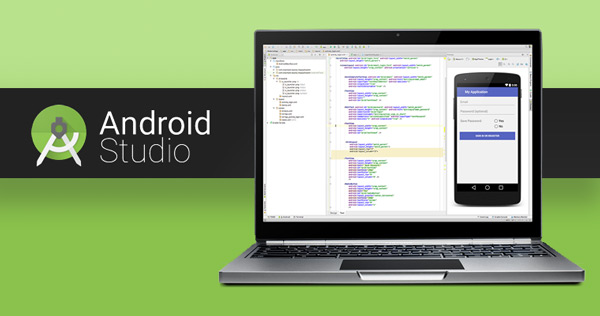
\includegraphics[width=0.6\linewidth]{androidstudio}
	\caption{Android Studio, un IDE flexible e intuitivo.}
	\label{fig:androidstudio}
\end{figure}

Se ha utilizado este IDE frente a otros como Eclipse + ADT \cite{URL::eclipseADT} debido a que en la actualidad es el IDE oficial con soporte de Google. Se ha preferido aprender a utilizar este entorno con vistas al futuro, ya que parece que se consolidará como el preferido para los desarrolladores Android.

\subsection{LaTex}

LaTeX es un sistema de composición de textos, orientado a la creación de documentos que presenten una alta calidad tipográfica. Por sus características y posibilidades, es usado especialmente en la generación de artículos y publicaciones científicas que incluyen, entre otros elementos, expresiones matemáticas, gráficos o figuras.


LaTeX está formado por un gran conjunto de macros de TeX, escrito por Leslie Lamport en 1984, con la intención de facilitar el uso del lenguaje de composición tipográfica, creado por Donald Knuth. LaTeX es software libre bajo licencia LPPL.


Se ha decidido utilizar este sistema debido al carácter profesional que aporta a los documentos. Ha sido una buena oportunidad para aprender a usar un sistema de composición de texto como este, ya que en un futuro puede ser beneficioso el saber manejar esta herramienta. 


Si bien es cierto, que el uso de esta herramienta frente a otros editores más familiares ha sido algo tedioso en el inicio, es verdad que una vez acostumbrada a su uso ha resultado ser muy eficaz. En el proceso de aprendizaje se recurrió principalmente a manuales por internet, alguno a destacar en español sería \cite{URL::manualLatex}

\subsection{Github}

GitHub\cite{URL::Github} es una forja (plataforma de desarrollo colaborativo) para alojar proyectos que utiliza el sistema de control de versiones Git. Utiliza el framework Ruby on Rails por GitHub, Inc. (anteriormente conocida como Logical Awesome). Desde enero de 2010, GitHub opera bajo el nombre de GitHub, Inc. El código se almacena de forma pública, aunque también se puede hacer de forma privada, creando una cuenta de pago.


Se ha decidido crear un repositorio en esta plataforma para poder llevar un control y una trazabilidad del proyecto. El tutor y el alumno han trabajado en este repositorio de manera conjunta. En el caso del tutor, principalmente para revisar el seguimiento semanal y llevar un control de las tareas. En el caso del alumno, para tener un repositorio donde subir los distintos elementos que se han ido generando a lo largo del trabajo. Aparte de este repositorio, también se ha abierto un segundo repositorio \cite{URL::repositorioAplicacion} asociado a la oficina del software libre (OSL) para subir el código una vez terminado como parte del programa de apoyo a trabajos finales libres (PATFL) \cite{URL::PATFL} de la ULL.


Mediante el uso de este repositorio, el alumno ha conseguido ampliar sus conocimientos en Git y familiarizarse con la interfaz de GitHub. Previamente se había utilizado como repositorios GitLab, SVN y RTC en otros proyectos, por lo que no ha sido una complicación mayor utilizar este sistema.

\section{Tecnologías utilizadas}

A continuación se revisan las distintas tecnologías utilizadas en el desarrollo de la aplicación.

\subsection{El Sistema Operativo Android}

Android es un sistema operativo que emplea Linux en la interfaz del hardware.  Los componentes del SO subyacentes se codifican en C o C++ pero las aplicaciones se desarrollan en Java. De esta manera Android asegura una amplia operatividad en una gran variedad de dispositivos debido a dos hechos: la interfaz en Linux ofrece gran potencia y funcionalidad para aprovechar el hardware, mientras que el desarrollo de las aplicaciones en Java permite que Android sea accesible para un gran número de programadores conocedores del código.

Este SO fue diseñado principalmente para dispositivos móviles con pantalla táctil: smartphones, tablets y otros dispositivos como televisores o automóviles. Fue desarrollado inicialmente por Android Inc., empresa que fue respaldada económicamente por Google y más tarde adquirida por esta misma empresa.

Actualmente tiene una gran comunidad de desarrolladores creando aplicaciones para extender la funcionalidad de los dispositivos. A fecha de hoy existen más de un millón de aplicaciones disponibles para la tienda oficial de Apps de Android, Google Play \cite{URL::GooglePlay} sin tener en cuenta las aplicaciones de otras tiendas no oficiales, como por ejemplo, la tienda de aplicaciones de Samsung Apps \cite{URL::SamsungApps}.

\subsection{AR}

La Realidad Aumentada(RA) o Augmented Reality(AR) en inglés es el término que se usa para definir la visión de un entorno físico del mundo real, a través de un dispositivo tecnológico. Este dispositivo, lo que hace es agregar elementos virtuales a una realidad existente, en lugar de crear esa realidad desde cero, como lo haría la realidad
virtual. 

 AR esta cambiando la manera en la que sus usuarios pueden ver el mundo, actualmente es una técnologia que se encuentra en auge sobre todo por el potencial que tendrá esta tecnologias en un futuro a largo y medio plazo. Sus posibles aplicaciones no tiene limites, puede llegar desde reconocer plantas e incluso monumentos y mostrar informacion sobre lo que se esta viendo , hasta añadir informacion en tiempo real en una operación a un paciente, comprobar como queda un mueble en tu salón o sus aplicaciones para realizar videojuegos como podemos ver con el recientce éxito de Pokemon Go!c

A continuacion se explicará en detalle:
\begin{itemize}
\item ¿Como funciona esta tecnologia?
\item Diferencias entre AR y VR
\item Futuro y usos de la AR
\item AR SDK en Android Studio
\end{itemize}  

\subsubsection{¿Como funciona esta tecnología?}
	
 En cuanto a la parte de hardware necesaria para poder hacer uso de esta tecnología necesitamos de un sistema de visualización, el cual puede ser una pantalla óptica transparente (Google Glass\cite{URL::GoogleGlass} )  o una pantalla de mezcla de imagenes(ej. pantalla de un móvil). 
\begin{figure}[h]
	\centering
	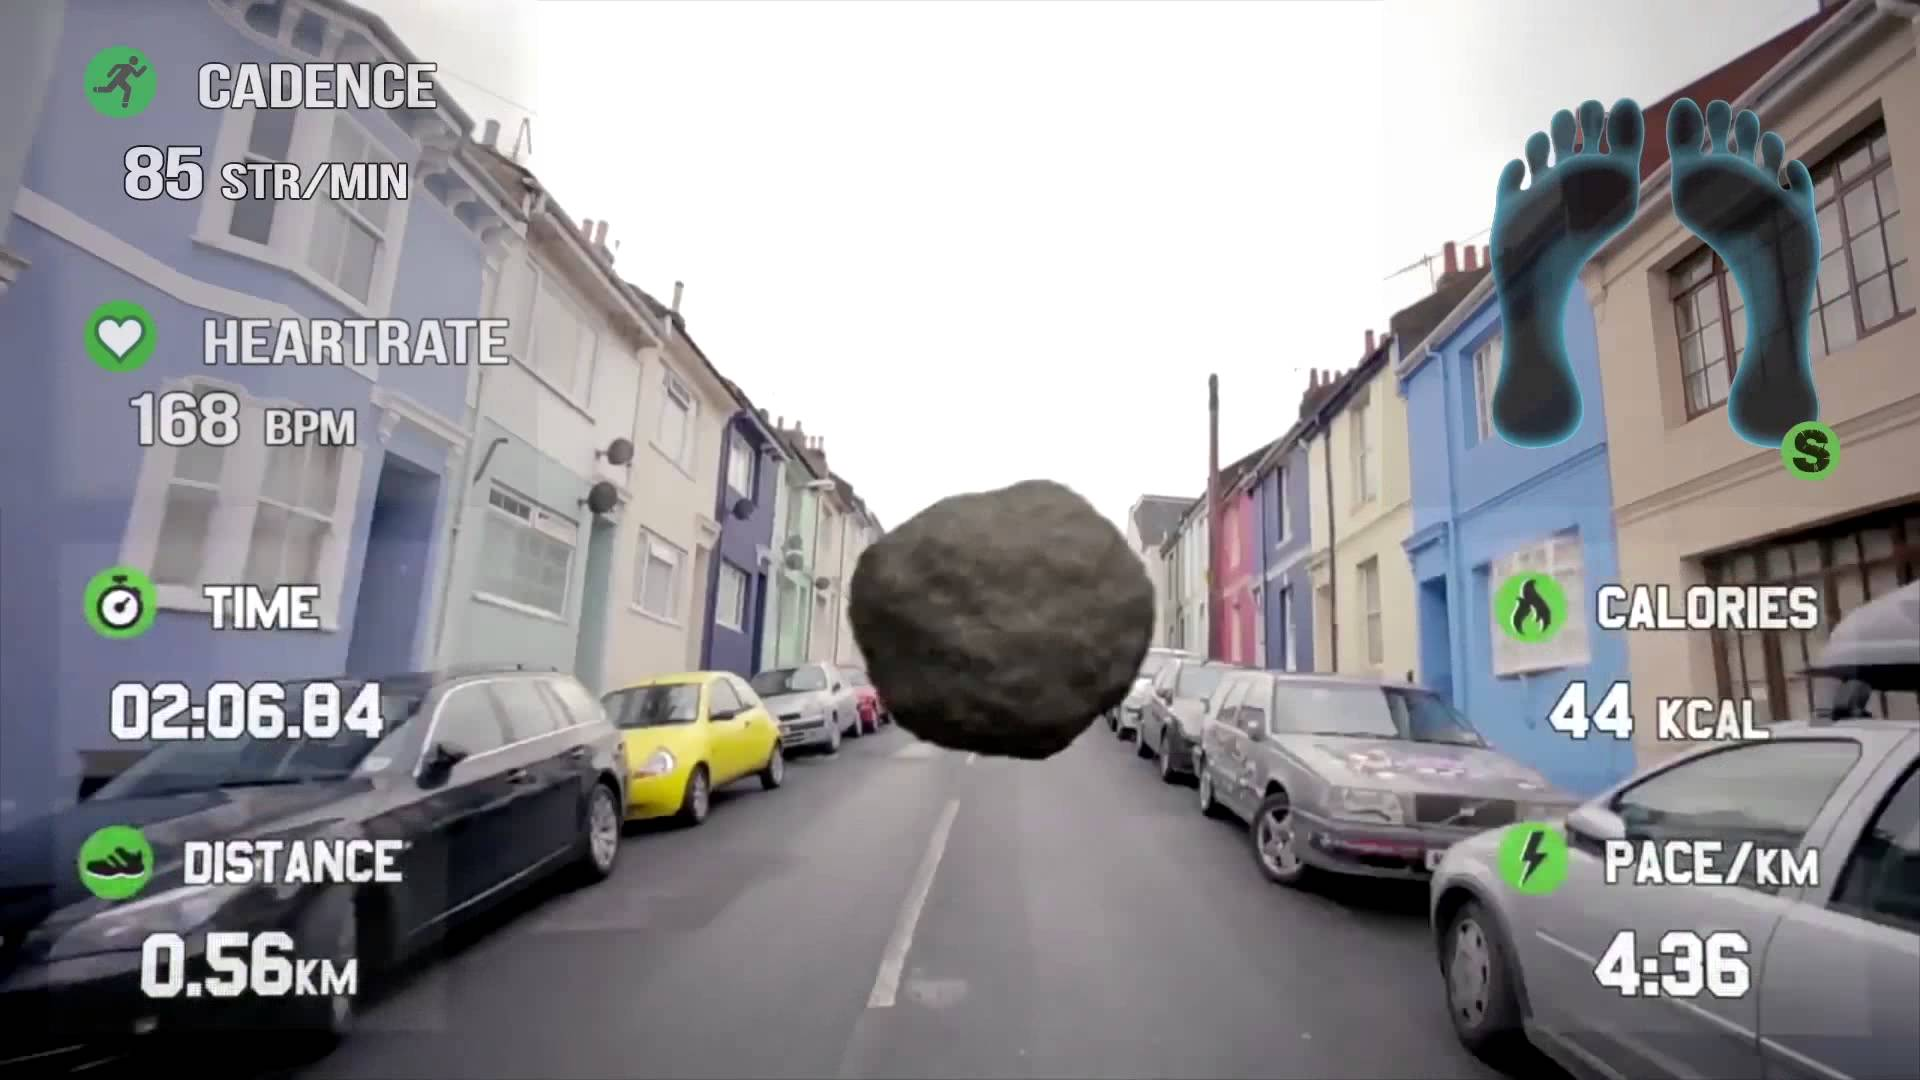
\includegraphics[width=0.6\linewidth]{googleglass}
	\caption{Google Glass. Desmostracion de su uso en deportes}
	\label{fig:googleglass}
\end{figure}
Además de esto sistemas de visualizacion, necesitaríamos de un sistema de computacion que realize los calculos y de otros sensores como el GPS\cite{URL::gps}, acelerometro, giroscopio, etc., que pese a nos ser estrictamente necesario, mejora la experiencia y las posibilidades de esta tecnologia.

Todo esto necesita una parte software la cual se encarga de hacer los calculos y de dar sentido la union de las imagenes obtenidas del mundo real junto a las imagenes virtuales a superponer en el mundo real.
 El software en una primera parte deberá de reconocer el terreno, ubicaciones, objetos e imagenes, mediante las imagenes obtenidas de la camara y los sensores. Este proceso de transformacion de diferentes conjuntos de datos a un sistema de coordenadas se llama registro de la imagen

y en una segunda reestructura el mundo real en función del registro de imagenes\cite{URL::ImageRegister} de del primer paso. Existen multiples maneras en las que se puede restructurar este mundo. 


\subsubsection{Diferencias entre AR y VR}
\subsubsection{Futuro y usos de la AR}
\subsubsection{AR SDK en Android Studio}

\subsubsection{Vuforia}

Es un SDK disponible para todas la plataformas(android, IOS, windows)y para Android Studio. Es muy potente para el desarrollo de aplicaciones de
realidad virtual, ya sea para el reconocimiento de imagenes, escanearlas, reconocimiento de multiples objetos, reconocimiento
y superficies planas. Ademas tambien permiten el reconocimento de acciones realizadas por el usuario para la interaccion con
los distintos elementos disponibles. El uso de esta SDK esta principalmente enfocado para trabajar junto Unity.


\subsubsection{Kudan}
Principal rival de Vuforia, facil de usar y eficiente, usa SLAM para el reconociento de objetos e imagenes
Tiene una licencia gratis para desarrolladores, una de sus desventajas es que tiene problemas con su key pare empezar a desarrollar y que a
veces tiene problemas con el editor de Unity.


\subsubsection{EasyAr}

En su version Free, tienes soporte para todas la plataformas y para Android Studio. Contiene reconocimento de imagenes planas, reconocimiento 
de imagenes multiples con deteccion de refleco y oclusion, reconocimiento limitado de imagenes en la nube.
    Su version mas potente se llama SLAM y solo es disponible para la version de pago.

  

\subsubsection{Maxst}

reconociento de objetos de imagenes, SLAM, multiplataforma, facil de usar. Optimizado para moviles, incluso con bajos recursos
Se puede utilizar con android studio, tienen un plan para desarrolladores free, con acceso a la mayoria de funcionalidades de su SDK


\subsection{Google Sheets}
\subsection{Google Maps}
